\subsection{Exercise 9 from TAOCP ``7.1.1 Boolean Basics'', solving it using Z3}

Page 34 from fasc0b.ps or \url{http://www.cs.utsa.edu/~wagner/knuth/fasc0b.pdf}.

\begin{figure}[H]
\label{fig:pipe_shuffled}
\centering
\frame{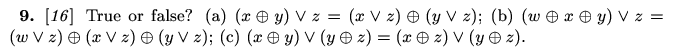
\includegraphics[scale=0.6]{FOL/TAOCP_7_1_1_exercise_9/fasc0b_page34.png}}
\caption{Page 34}
\end{figure}

For (a):

\lstinputlisting{FOL/TAOCP_7_1_1_exercise_9/Knuth_a.smt}

For (b):

\lstinputlisting{FOL/TAOCP_7_1_1_exercise_9/Knuth_b.smt}

For (c):

\lstinputlisting{FOL/TAOCP_7_1_1_exercise_9/Knuth_c.smt}

Results:

\lstinputlisting{FOL/TAOCP_7_1_1_exercise_9/results.txt}

